\section{Méthodologie}
\label{sec:methodologie}

Nous présentons ici le déroulement de nos expérimentations qui consistent à étudier le phénomène du renommage et son impact sur le calcul des métriques de procédés. L’objectif étant d’évaluer si le renommage peut biaiser de manière significative les valeurs des métriques de procédés.\\

Le but de la première expérience et de calculer la quantité de renommage durant les périodes de développement. S’appuyant sur cette première expérience, notre deuxième expérience fournit une analyse de l’impact du renommage sur les métriques de procédés dans le pire des cas. \\

\subsection{Corpus}

Nous avons sélectionné un ensemble de projets sur lesquels effectuer nos expérimentations qui respectent le modèle défini. Des projets open-source, conséquents et connues de la communauté MSR. Nous avons un ensemble de projets utilisés par l'équipe de Génie Logiciel au LaBRI qui respectent le modèle avec des branches de maintenances identifiées. Les $5$ projets qui sont donnés \tabref{projects} forment un corpus pour notre prochaine expérience. Il comprend différents langages de programmation ainsi qu'un nombre de lignes de code et un nombre de développeurs moyennement élevés à évélevés par rapport aux projets open source utilisés couramment par la communauté. Les $5$ projets sont gérés sur Git afin de profiter de la détection automatique des renommages (section). 

De plus, il faut noter que nous avons choisi d'exclure tous les fichiers qui ne sont pas du code source du corpus étant donné que les métriques de procédés sont habituellement uniquement calculées sur ces fichiers. \\

\begin{table*}[h]
\centering
\small
\begin{tabular}{rllp{1.7cm}c}
\toprule
Project & Main language & Size (LoC) & Number of developers & URL\\
\midrule
Jenkins & Java & 200851 & 454 & \url{github.com/jenkinsci/jenkins} \\
JQuery & JavaScript & 41656 & 223 & \url{github.com/jquery/jquery} \\
PHPUnit & PHP & 21799 & 152 & \url{github.com/sebastianbergmann/phpunit}\\
Pyramid & Python & 38726 & 205 & \url{github.com/Pylons/pyramid} \\
Rails & Ruby & 181002 & 2767 & \url{github.com/rails/rails}\\
\bottomrule
\end{tabular}
\caption{Notre corpus de projets.}
\label{tab:projects}
\end{table*}

\subsection{Première expérience}

Nous définissons maintenant le modèle \figref{model}, que les projets que nous allons analyser devrons respecter. Ce modèle représente une architecture pour le dépôt de code source dérivé de l'architecture Git Flow.\\

\begin{figure}[h]
  \centering
  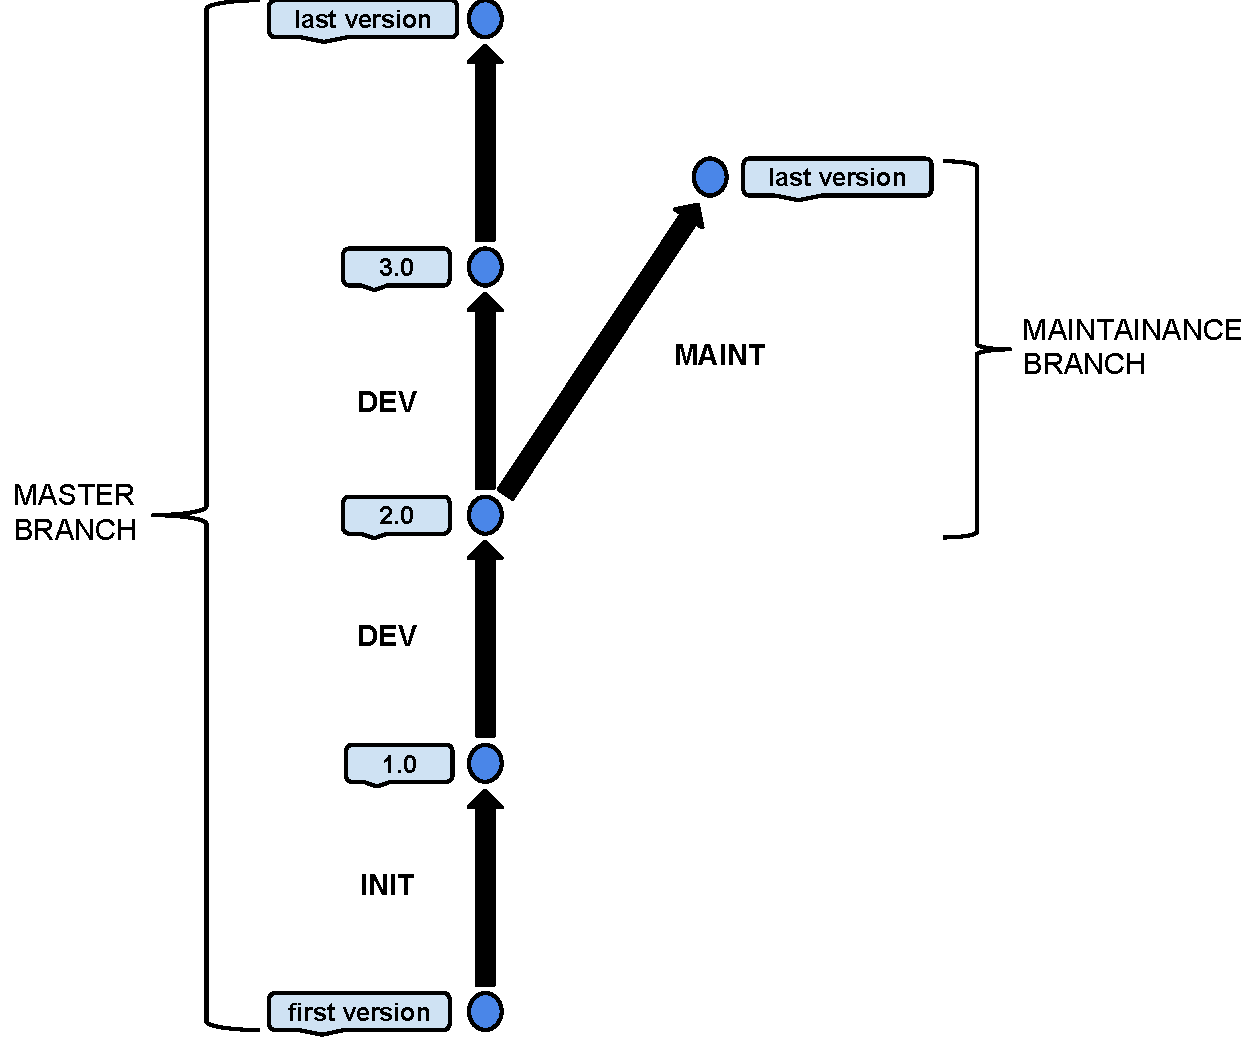
\includegraphics[scale=0.5]{data/figures/periods.pdf}
	\caption{Modèle d'architecture de dépot de code source}
	\label{fig:model}
\end{figure}

Les projets de développement logiciel suivent généralement des phases distinctes durant leur cycle de vie. Habituellement une période de développement commence avant qu'une première release soit accessible aux utilisateurs, puis cette release est maintenue pendant qu'une autre se prépare et ainsi de suite.

Nous avons ainsi deux types de branches, les branches de maintenance et la branche master. Nous divisons les branches en périodes, c'est-à-dire en une séquence de commits, la branche master contient une période initiale (init) entre la première version du logiciel (incluse) et la première release, puis des périodes de développement (dev) entre chaque release. Chaque projet contient des releases majeures, qui correspondent à des points-clés du projet, des périodes susceptibles de contenir beaucoup de changements, et des releases mineures. On distingue les releases majeures des mineures par une augmentation significative du numéro de release. Par exemple $1.9-2.0$ pour Jquery, $3.7-4.0$ pour PHPUnit ou $0.13-1.0$ pour Rails. De l'autre côté les branches de maintenance sont divisées en périodes (maint) entre chaque release.\\

 L'objectif de notre première expérience est de mieux comprendre le renommage d'entités. En particulier, d'observer quand les renommages apparaissent et en quelle quantité. Nous avons donc analysé chaque période comme décrites précédemment sur chaque projet de notre corpus. Nous comptons donc sur la détection automatique de renommage de Git et l'utilisons dans notre outil développé en Ruby pour obtenir nos chiffres (détails dans la section résultats). (TODO pourquoi Ruby ?) Nous suivons ces trois étapes entre chaque période:
\begin{enumerate}
\item On liste les fichiers existant à la fin de la période.
\item Pour chacun de ces fichiers, on extrait sa séquence de modification durant la période en activant la détection de renommage (commande \texttt{git log -M})
\item On calcule à partir des informations receuillies. Par exemple le pourcentage de fichiers $\%F_{R}$ qui ont été renommés au moins une fois durant la période.
\end{enumerate}
\medskip

À notre connaissance, il n'existe pas d'évaluation empirique de l'algorithme utilisé par Git pour détecter les renommages. Néanmoins, nous procédons à une évaluation manuelle de son comportement dans la partie conclusion et nous n'avons pas noté de faux positif sur 100 renommages aléatoire récupérés par notre outil.\\

\subsection{Deuxième expérience}

L'objectif de la deuxième expérience est de voir si le renommage peut biaiser significativement les valeurs des métriques de procédés décrites ci-dessus. Pour ça, nous effectuons une analyse dans le pire des cas.(TODO expliquer ?) On sélectionne la période de nos projets qui a la plus grande valeur de fichiers renommés en excluant la période initiale qui n'est généralement pas observée dans les études. Nous calculons ensuite les trois métriques avec et sans le renommage de fichiers pris en compte, puis nous calculons la corrélation de coefficient de Spearman entre les métriques avec et sans la détection de renommage. Un coefficient élevé, proche de $1$, indiquera que les métriques avec et sans détection de renommage sont très similaires alors qu'un coefficient plus petit, 0.5 et moins, indiquera que les métriques avec et sans détection de renommage sont très différentes.\\  
